\documentclass[letterpaper,11pt]{article}

\usepackage{latexsym}
\usepackage[empty]{fullpage}
\usepackage{titlesec}
\usepackage{marvosym}
\usepackage[usenames,dvipsnames]{color}
\usepackage{verbatim}
\usepackage{enumitem}
\usepackage[hidelinks]{hyperref}
\usepackage{fancyhdr}
\usepackage[english]{babel}
\usepackage{tabularx}
\usepackage{fontawesome5}
\usepackage{multicol}
\setlength{\multicolsep}{-3.0pt}
\setlength{\columnsep}{-1pt}
\input{glyphtounicode}

%new packages

\usepackage{fontenc}
\usepackage{amsmath}
\usepackage{amssymb}
\usepackage{graphicx}



%----------FONT OPTIONS----------

\pagestyle{fancy}
\fancyhf{} % clear all header and footer fields
\fancyfoot{}
\renewcommand{\headrulewidth}{0pt}
\renewcommand{\footrulewidth}{0pt}

% Adjust margins
\addtolength{\oddsidemargin}{-0.6in}
\addtolength{\evensidemargin}{-0.5in}
\addtolength{\textwidth}{1.19in}
\addtolength{\topmargin}{-.7in}
\addtolength{\textheight}{1.4in}

\urlstyle{same}

\raggedbottom
\raggedright
\setlength{\tabcolsep}{0in}

% Sections formatting
\titleformat{\section}{
  \vspace{-4pt}\scshape\raggedright\large\bfseries
}{}{0em}{}[\color{black}\titlerule \vspace{-5pt}]



% Ensure that generate pdf is machine readable/ATS parsable
\pdfgentounicode=1

%-------------------------
% Custom commands
\newcommand{\resumeItem}[1]{
  \item\small{
    {#1 \vspace{-2pt}}
  }
}

\newcommand{\classesList}[4]{
    \item\small{
        {#1 #2 #3 #4 \vspace{-2pt}}
  }
}

\newcommand{\resumeSubheading}[4]{
  \vspace{-2pt}\item
    \begin{tabular*}{1.0\textwidth}[t]{l@{\extracolsep{\fill}}r}
      \textbf{#1} & \textbf{\small #2} \\
      \textit{\small#3} & \textit{\small #4} \\
    \end{tabular*}\vspace{-7pt}
}

\newcommand{\resumeSubSubheading}[2]{
    \item
    \begin{tabular*}{0.97\textwidth}{l@{\extracolsep{\fill}}r}
      \textit{\small#1} & \textit{\small #2} \\
    \end{tabular*}\vspace{-7pt}
}

\newcommand{\resumeProjectHeading}[2]{
    \item
    \begin{tabular*}{1.001\textwidth}{l@{\extracolsep{\fill}}r}
      \small#1 & \textbf{\small #2}\\
    \end{tabular*}\vspace{-7pt}
}


\newcommand{\resumeSubItem}[1]{\resumeItem{#1}\vspace{-4pt}}

\renewcommand\labelitemi{$\vcenter{\hbox{\tiny$\bullet$}}$}
\renewcommand\labelitemii{$\vcenter{\hbox{\tiny$\bullet$}}$}

\newcommand{\resumeSubHeadingListStart}{\begin{itemize}[leftmargin=0.0in, label={}]}
\newcommand{\resumeSubHeadingListEnd}{\end{itemize}}
\newcommand{\resumeItemListStart}{\begin{itemize}}
\newcommand{\resumeItemListEnd}{\end{itemize}\vspace{-5pt}}


\begin{document}
\fontfamily{cmr}\selectfont
\begin{center}
\parbox{3.0cm}{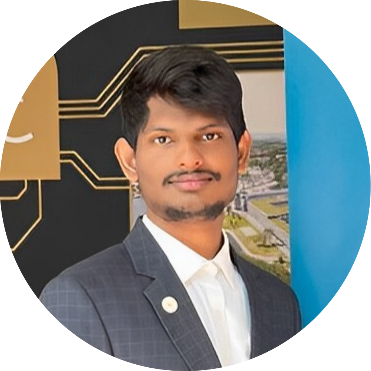
\includegraphics[width=2.7cm,clip]{images/resume_pic_m.png}}
\parbox{\dimexpr\linewidth-3.8cm\relax}{
\vspace{-20pt}
\begin{tabularx}{\linewidth}{L r} \\
    {\Huge \scshape  Venkata Sai Yakkshit Reddy Asodi}~
    \href{https://www.cedzlabs.com/yakkshit}{\vspace{1pt}}\\
      Berlin, Germany. \\ \vspace{1pt}
     \small \raisebox{-0.1\height}\faPhone\ +91 8179936156 ~ \href{mailto:saiyakkshit2001@gmail.com}{\raisebox{-0.2\height}\faEnvelope\  {saiyakkshit2001@gmail.com}} ~ 
    \href{https://linkedin.com/in/yakkshit/}{\raisebox{-0.2\height}\faLinkedin\ {yakkshit}}  ~
    \href{https://yakkshit.com/}{\raisebox{-0.2\height}\faGlobe\ {yakkshit.com}}  ~
    \href{https://github.com/yakkshit}{\raisebox{-0.2\height}\faGithub{ yakkshit}}
    \vspace{-8pt}
    
\end{tabularx}
}
\end{center}

\vspace{-23pt}
\section{Summary}
Dynamic Full Stack Developer with expertise in React.js, Next.js, Node.js, and MongoDB. Experience in building innovative, scalable web applications and APIs. Passionate about mental health and leveraging technology to build impactful online platforms. Fluent in Agile methodologies and always eager to learn new technologies.

\section{Technical Skills}
\begin{itemize}[leftmargin=0.15in, label={}]
\small{\item{
\textbf{Frontend - }{React.js, Next.js, TailwindCSS, HTML5, CSS3.} \\
\textbf{Backend - }{Node.js, MongoDB, RESTful APIs.} \\
\textbf{Cloud - }{AWS, Docker, CI/CD pipelines.} \\
\textbf{Tools - }{Git, Postman, Swagger.} \\
}}
\end{itemize}
\vspace{-10pt}

\section{Experience}

\resumeSubHeadingListStart
\resumeSubheading
{\large Circleup AG}{December 2023 -- July 2024}
  {Lead Full Stack Engineer}{Zurich, Switzerland}\\
\vspace{10pt}
\textbf{Responsibilities:}
\resumeItemListStart
\resumeItem{Developed scalable web applications using React.js and integrated with Django-based APIs.}
\resumeItem{Led front-end development of the event scheduling platform, ensuring smooth user experiences across devices.}
\resumeItem{Collaborated with backend teams to build and enhance API endpoints using Django.}
\resumeItemListEnd
\vspace{-3pt}

\resumeSubheading
{\large Cedzlabs}{March 2023 -- July 2024}
{Full Stack Developer}{India}\\
\vspace{10pt}
\textbf{Responsibilities:}
\vspace{-10pt}
\resumeItemListStart
\resumeItem{Created an intuitive UI for a multilingual chat app using React.js and Next.js.}
\resumeItem{Worked closely with cross-functional teams to gather requirements and deploy features.}
\resumeItemListEnd
\vspace{-3pt}

\resumeSubHeadingListEnd

\section{Projects}
\vspace{-5pt}
\resumeSubHeadingListStart

\resumeProjectHeading
{\textbf{\href{https://ui.cedzlabs.com/resume}{AI Resume Tuner}} $|$ \emph{Next.js, Azure, RAG}}{August 2023}\\
\vspace{6pt}
\textbf{Description:}
\resumeItemListStart
\resumeItem{Built an AI-powered resume generator using Retrieval Augmented Generation (RAG) and deployed it on Azure Cloud. The project helps users generate customized resumes based on job descriptions.}
\resumeItemListEnd
\vspace{4pt}

\resumeProjectHeading
{\href{https://yakkshit.com}{\textbf{Portfolio Website}} $|$ \emph{Next.js, AWS}}{January 2023}\\
\vspace{6pt}
\textbf{Description:}
\vspace{-5pt}
\resumeItemListStart
\resumeItem{Designed and implemented a secure portfolio website using Next.js and deployed it on AWS with a focus on accessibility and performance.}
\resumeItemListEnd
\vspace{4pt}

\resumeSubHeadingListEnd

\section{Achievements}
\vspace{-5pt}
\resumeSubHeadingListStart
\resumeItemListStart
\resumeItem{Contributed to open-source projects in the web development space.}
\resumeItem{Participated in Microsoft Hackathon to develop an AI-powered resume generator.}
\resumeItemListEnd
\resumeSubHeadingListEnd

\textbf{Languages:} Telugu - Native $|$ English - Fluent $|$ German - Elementary.

\end{document}